%%%%%%%%%%%%%%%%% DO NOT CHANGE HERE %%%%%%%%%%%%%%%%%%%% {
\documentclass[10pt,a4]{article}
\DeclareMathSizes{10}{10}{5.5}{4}
\usepackage{enumerate}
\usepackage{xcolor}
\usepackage{graphicx}
\usepackage{listings}
\usepackage{hyperref}
\usepackage{ctex}
\usepackage{tikz}
\usepackage{geometry}%页边距调整
\geometry{left=2cm,right=2cm,bottom=2.8cm,top=2cm}
\usepackage{newtxtext}
\usepackage{newtxmath,bm}
\usepackage{titlesec}
\usepackage{fancyhdr}
\usepackage{booktabs}
\usepackage{makecell}

\definecolor{titlepurple}{HTML}{5758BB}%一级标题(目前:蓝紫色)
\definecolor{titlepurpleb}{HTML}{3A006F}%二级标题(目前:深紫色)
\definecolor{titlepurplec}{HTML}{006266}%三级标题(目前:墨绿色)
\definecolor{tab1}{HTML}{9698ED}%表格1
\definecolor{tab2}{HTML}{DBDCFF}%表格2
\definecolor{dy0}{HTML}{EA7500}%小标题定义专用(目前:橙黄色)
\definecolor{dl}{HTML}{007500}%小标题定理专用(目前:深绿色)
\definecolor{inference}{HTML}{343300}%小标题推论专用(目前:墨绿色)
\definecolor{ex}{HTML}{7158e2}%小标题例专用(目前:紫色)
\definecolor{dy}{HTML}{BF0060}%夹杂在文本中的定义词的颜色1(目前:深红色)
\definecolor{dy2}{HTML}{FF0000}%夹杂在文本中的定义词的颜色2(目前:红紫色)
\definecolor{dya}{HTML}{FFFFFF}
\definecolor{超链接}{HTML}{0000C6}%含超链接的文字专用色(目前:蓝紫色)
\definecolor{文字底色}{HTML}{F8FF00}%强调的文字底色(目前:黄色)
\definecolor{eq}{HTML}{F0F0F0}
\definecolor{tl}{HTML}{D94600}

\titleformat{\section}{\bfseries\Large\color{titlepurple}}{第 \ \thesection\  章\quad }{0pt}{}
\titleformat{\subsection}{\large\bfseries\color{titlepurplec}}{\thesubsection\ \quad  }{0pt}{}
\titlespacing{\subsection}{0em}{0.1em}{0.3em}[1em]
%格式如下:\titlespacing*{章节名称}{左间距}{(前)行间距}{(后)行间距}[右间距(一般都没用,填0.1em即可,但不能不填)]
\titlespacing*{\subsubsection}{1.5em}{0.5em}{0.3em}[0em]
\numberwithin{equation}{section}

\hypersetup{%
  colorlinks=true,
  linkcolor=blue,
  linkbordercolor={0 0 1}
}

\setCJKmainfont[BoldFont={PingFangSC-Medium}]{PingFangSC-Regular}
\setlength{\parindent}{0.0in}
\setlength{\parskip}{0.05in}
%%%%%%%%%%%%%%%%%%%%%%%%%%%%%%%%%%%%%%%%%%%%%%%%%%%%%%%%%% }

% %%%%%%%%%%%%%%%%%%%%%%%% CHANGE HERE %%%%%%%%%%%%%%%%%%%% {
% %Margins and Header/Footer
% \geometry{a4paper,
%   top=2in,
%   bottom=1.5in,
%   left=1.5in,
%   right=1in,
%   headheight=14.5pt, % the default is too short
%   heightrounded, % avoids the need of a flexible baselineskip
% } 
% %%%%%%%%%%%%%%%%%%%%%%%%%%%%%%%%%%%%%%%%%%%%%%%%%%%%%%%%%% }

%%%%%%%%%%%%%%%%%%%%%%%% CHANGE HERE %%%%%%%%%%%%%%%%%%%% {
\newcommand\course{\Large \textcolor[rgb]{0.12,0.33,0.12}{\textbf{轨道力学}}}
\newcommand\semester{\large \textcolor[rgb]{0.12,0.33,0.12}{2021 年秋季学期}}
\newcommand\SchoolLogo{
\includegraphics[scale=0.35]{./pic/SYSU_SAA_Logo.pdf}}
%%%%%%%%%%%%%%%%%%%%%%%%%%%%%%%%%%%%%%%%%%%%%%%%%%%%%%%%%% }

%%%%%%%%%%%%%%%%% DO NOT CHANGE HERE %%%%%%%%%%%%%%%%%%%% {
\pagestyle{fancyplain}
\headheight 30pt
\rhead{	
	\quad \\[1em]
	\begin{minipage}[l]{0.39\linewidth}
		\hspace*{-1em}
		\SchoolLogo
	\end{minipage}
	\begin{minipage}[r]{0.6\linewidth}
	\vspace*{0.4em}\makecell[r]{\course \\[0.3em] \semester}
\end{minipage}\\[-1.1em]} 
\setlength{\headsep}{3.5em}
\setlength{\footskip}{2.5em}
\renewcommand{\headrulewidth}{0mm}
\rfoot{\textcolor[rgb]{0.12,0.33,0.12}{\small \bfseries 轨道力学笔记}}
\cfoot{\textcolor[rgb]{0.12,0.33,0.12}{\small \bfseries \thepage}} 
\lfoot{\textcolor[rgb]{0.12,0.33,0.12}{\small \bfseries 2019级航空航天工程专业本科}} 

\renewcommand{\d}{\text{d}}
\def\degree{{}^{\circ}}
%%%%%%%%%%%%%%%%%%%%%%%%%%%%%%%%%%%%%%%%%%%%%%%%%%%%%%%%%% }

\title{\huge \bf
	轨道力学笔记
}
\author{19320125 \hspace*{1em} 易鹏}

\begin{document}
\maketitle

\section{质点运动学}

\section{二体问题}
\subsection{惯性系的运动方程}
\subsubsection{质心$G$的运动物理量}
\begin{equation}
	\mbox{质心} G \, 
	\begin{cases}
		\, \mbox{位置矢量} & \bm{R}_G = \dfrac{m_1 \bm{R}_1 + m_2 \bm{R}_2}{m_1 + m_2}\\[1em]
		\, \mbox{速度} & \bm{v}_G = \dfrac{m_1 \dot{\bm{R}}_1 + m_2 \dot{\bm{R}}_2}{m_1 + m_2}\\[1em]
		\, \mbox{加速度} & \bm{a}_G = \dfrac{m_1 \ddot{\bm{R}}_1 + m_2 \ddot{\bm{R}}_2}{m_1 + m_2}
	\end{cases}
\end{equation}

\subsubsection{质心$G$与惯性系原点}
\hspace*{2em} 记相对位置矢量为$\bm{r} = \bm{R}_2 - \bm{R}_1$,单位化为$\widehat{\bm{u}}_r$由牛顿第二定律,
\begin{equation*}
	\begin{cases}
		\bm{F}_{21} = \dfrac{Gm_1m_2}{r^2}\cdot (-\widehat{\bm{u}}_r) = m_2 \ddot{\bm{R}}_2\\[0.8em]
		\bm{F}_{12} = \dfrac{Gm_1m_2}{r^2}\cdot (\widehat{\bm{u}}_r) = m_1 \ddot{\bm{R}}_1
	\end{cases}
\end{equation*}
所以
\begin{equation}
	m_1 \ddot{\bm{R}}_1 + m_2 \ddot{\bm{R}}_2 = 0 \quad \Rightarrow \quad \bm{a}_G = 0 \quad \Rightarrow \quad \mbox{质心可作为惯性坐标系原点} \quad \Rightarrow \quad \bm{R}_G = \bm{R}_{G_0} + \bm{v}_G t
\end{equation}

\subsection{相对运动方程}
\begin{equation}
	\ddot{\bm{r}} = - \dfrac{\mu}{r^3}\bm{r}\quad \mu = G(m_1 + m_2)
\end{equation}
有类似的结果
\begin{equation}
	\begin{cases}
		\, \ddot{\bm{r}}_2 = - \dfrac{\mu'}{r^3}\cdot \bm{r}_2 \quad \mu' = \left(\dfrac{m_1}{m_1 + m_2}\right)^3\cdot \mu \\[0.8em]
		\, \ddot{\bm{r}}_2 = - \dfrac{\mu''}{r^3}\cdot \bm{r}_2 \quad \mu'' = \left(\dfrac{m_2}{m_1 + m_2}\right)^3\cdot \mu
	\end{cases}
\end{equation}
其原因为
\begin{equation}
	\ddot{\bm{r}} = \ddot{\bm{r}}_{\mbox{\scriptsize 相对}} + \dot{\bm{\Omega}} \times \bm{r} + \bm{\Omega}\times(\bm{\Omega}\times \bm{r}) + 2 \bm{\Omega}\times \dot{\bm{r}}_{\mbox{\scriptsize 相对}}
\end{equation}

$\ddot{\bm{r}} = \ddot{\bm{r}}_{\mbox{\scriptsize 相对}}  $当且仅当$\bm{\Omega} = \dot{\bm{\Omega}} = 0$
$\quad \longrightarrow  \quad$运动坐标系为非旋转坐标系时,$\ddot{\bm{r}}$可以用$\bm{r}_{\scriptsize\mbox{相对}}$$\quad \longrightarrow  \quad$ 二体问题中的任一物体相对于质心的运动方程有相同的形式。
\vspace*{0.5em}

\subsection{角动量和轨道方程}
\subsubsection{角动量的定义}
\hspace*{2em} $m_2$相对于$m_1$的角动量为
\begin{equation}
	H_{12} = \bm{r} \times m_2 \dot{\bm{r}}
\end{equation}
定义比角动量为
\begin{equation}
	\bm{h} = \bm{r} \times \dot{\bm{r}} = h \cdot \hat{\bm{h}}
\end{equation}

\subsubsection{角动量的性质}
1. 两体问题中角动量不变
\begin{equation}
	\dfrac{\d \bm{h}}{\d t} = \bm{r} \times \left(-\dfrac{\mu}{r^3} \bm{r}\right) = 0
\end{equation}

\noindent 2. 角动量的大小仅取决于相对速度的垂直分量
\begin{equation}
	\bm{h} = r v_{\bot}\cdot \hat{\bm{h}}
\end{equation} 

\noindent 3. 开普勒第二定律
\begin{equation}
	\d A = \dfrac{1}{2} v \, \d t  \cdot r\sin \phi = \dfrac{1}{2}r(v \sin \phi )\d t = \dfrac{1}{2} r v_{\bot}\d t  \quad \Rightarrow \quad \dfrac{\d A}{\d t} = \dfrac{h}{2}
\end{equation}

\subsubsection{轨道方程}
矢量方程$\bm{r}$
\begin{equation}
	\dfrac{\bm{r}}{r} + \bm{e} = \dfrac{\dot{\bm{r}}\times \bm{h}}{\mu}
\end{equation}
标量方程$r$
\begin{equation}
	r = \dfrac{h^2}{\mu} \dfrac{1}{1 + e \cos \theta}
\end{equation}
速度$\bm{v}$
\begin{equation}
	\begin{cases}
		\, v_{\bot} = \dfrac{h}{r} = r^2 \dot{\theta} = \dfrac{\mu}{h}(1 + e \cos \theta)\\[0.8em]
		\, v_r = \dfrac{\d r}{\d t} = \dfrac{\mu}{h}e \sin \theta
	\end{cases}
	\quad \Rightarrow \quad v^2 = v_r^2 + v_{\bot}^2 = \dfrac{\mu^2}{h^2}(e^2 + 2e\cos \theta + 1)
\end{equation}
飞行速度角$\gamma$
\begin{equation}
	\tan \gamma = \dfrac{v_r}{v_{\bot}} = \dfrac{e \sin \theta}{1 + e \cos \theta}
\end{equation}
近地点
\begin{equation}
	\theta = 0: \,
	\begin{cases}
		\, r_p = \dfrac{h^2}{\mu} \dfrac{1}{1 + e}\\
		\, v_r = 0
	\end{cases}
\end{equation}
半通径$p$
\begin{equation}
	p = \dfrac{h^2}{\mu}
\end{equation}

\subsection{能量定律}
能量定义
\begin{equation}
	\varepsilon = \dfrac{v^2}{2} - \dfrac{\mu}{r} = \dfrac{1}{2} \dfrac{\mu^2}{h^2}(e^2 - 1)
\end{equation}

\subsection{小结}
\hspace*{2em}轨道方程$r = \dfrac{h^2}{\mu} \, \longrightarrow \, \mbox{参数}h,\mu,e,\theta,p \, \longrightarrow \, \,
\begin{cases}
	\, \mbox{近地点}\\
	\, \mbox{拱线}\\
	\, \mbox{飞行路径角}
\end{cases} \, \longrightarrow \, \mbox{能量定律:}\varepsilon = \dfrac{v^2}{2} - \dfrac{\mu}{r} =\dfrac{1}{2} \dfrac{\mu^2}{h^2}(e^2 - 1)$

\subsection{圆轨道($e = 0$)}
\begin{table}[!htb]
	\centering
	\setlength{\tabcolsep}{8mm}{
		\begin{tabular}{clcl}
			\hline
			&&&\\[-1.2em]
			轨道半径 & $\displaystyle r = \dfrac{h^2}{\mu}$ & 速度 & $\displaystyle v = v_{\bot} = \dfrac{h}{r} = \dfrac{\mu}{h}$ \\
			&&&\\[-1.2em]
			\hline
			&&&\\[-1.2em]
			径向速度 & $v_r = 0$ & 切向速度 & $v_{\bot} = \dfrac{h}{r} = \dfrac{\mu}{h}$ \\
			&&&\\[-1.2em]
			\hline
			&&&\\[-1.1em]
			轨道周期 & $\displaystyle T = \dfrac{2 \pi r}{v} = \dfrac{2 \pi r h}{\mu} = \dfrac{2 \pi}{\sqrt{\mu}} \cdot  r^{\textstyle \frac{3}{2}}$ & 轨道能量 & $\varepsilon = -\dfrac{1}{2} \dfrac{\mu}{h^2} = - \dfrac{\mu}{2r}$ \\[0.7em]
			\hline
		\end{tabular}
	}
	\caption{圆轨道的各个参数}
	\label{圆1}
\end{table}

\subsection{椭圆轨道($0 < e < 1$)}

\begin{table}[!htb]
	\centering
	\setlength{\tabcolsep}{3.5mm}{
		\begin{tabular}{clcl}
			\hline
			&&&\\[-1.2em]
			远地点 & $\displaystyle r_a = \dfrac{h^2}{\mu} \dfrac{1}{1 - e} = a (1 + e)$ & 近地点 & $\displaystyle r_p = \dfrac{h^2}{\mu} \dfrac{1}{1 + e} = a (1 - e)$ \\
			&&&\\[-1.2em]
			\hline
			&&&\\[-1.2em]
			短半轴 & $\displaystyle a = \dfrac{r_a + r_p}{2} = \dfrac{h^2}{\mu} \dfrac{1}{1 -e^2}$ & 长半轴 & $\displaystyle b = a \sqrt{1 - e^2}$ \\
			&&&\\[-1.2em]
			\hline
			&&&\\[-0.8em]
			离心率 & $\displaystyle e = \dfrac{r_a - r_p}{r_a + r_p}$ & 飞行路径角  &  $\displaystyle \tan \gamma =  \dfrac{e \sin \theta}{1 + e \cos \theta}$ \\
			&&&\\[-1.3em]
			\hline
			&&&\\[-1.2em]
			轨道半径 & $\displaystyle r = \dfrac{h^2}{\mu} \dfrac{1}{1 + e \cos \theta} = \dfrac{a(1-e^2)}{1 + e \cos \theta}$ & 速度 & $\displaystyle  v^2 = v_r^2 + v_{\bot}^2 = \dfrac{\mu^2}{h^2}(e^2 + 2e\cos \theta + 1)$ \\
			&&&\\[-1.2em]
			\hline
			&&&\\[-0.8em]
			径向速度 & $\displaystyle v_r =  \dfrac{\mu}{h}e \sin \theta$ & 切向速度 & $\displaystyle  v_{\bot} = \dfrac{\mu}{h}(1 + e \cos \theta)$ \\
			&&&\\[-1em]
			\hline
			&&&\\[-1.1em]
			轨道周期 & $\displaystyle T = \dfrac{\Delta A}{h/2} = \dfrac{2 \pi ab}{h} = 2 \pi \left(\dfrac{h}{\sqrt{1 - e^2}}\right)^3 = \dfrac{2 \pi }{\sqrt{\mu}} a ^{\textstyle \frac{3}{2}}$ & 轨道能量 & $\varepsilon = -\dfrac{1}{2} \dfrac{\mu}{h^2}(1 - e^2) = - \dfrac{\mu}{2a}$ \\[0.9em]
			\hline
		\end{tabular}
	}
	\caption{椭圆轨道的各个参数}
	\label{椭圆1}
\end{table}

\hspace*{2em}$m_1,m_2$在整个运动周期内的平均距离为
\begin{equation}
	\overline{r} = a \sqrt{1 - e^2} = \sqrt{r_a r_p} = b
\end{equation}
将真近点角平分$n$等分,空间上的平均。

\clearpage
\quad \\[-5em]
\begin{figure}[!htb]
	\begin{minipage}{0.55\linewidth}
		\centering
		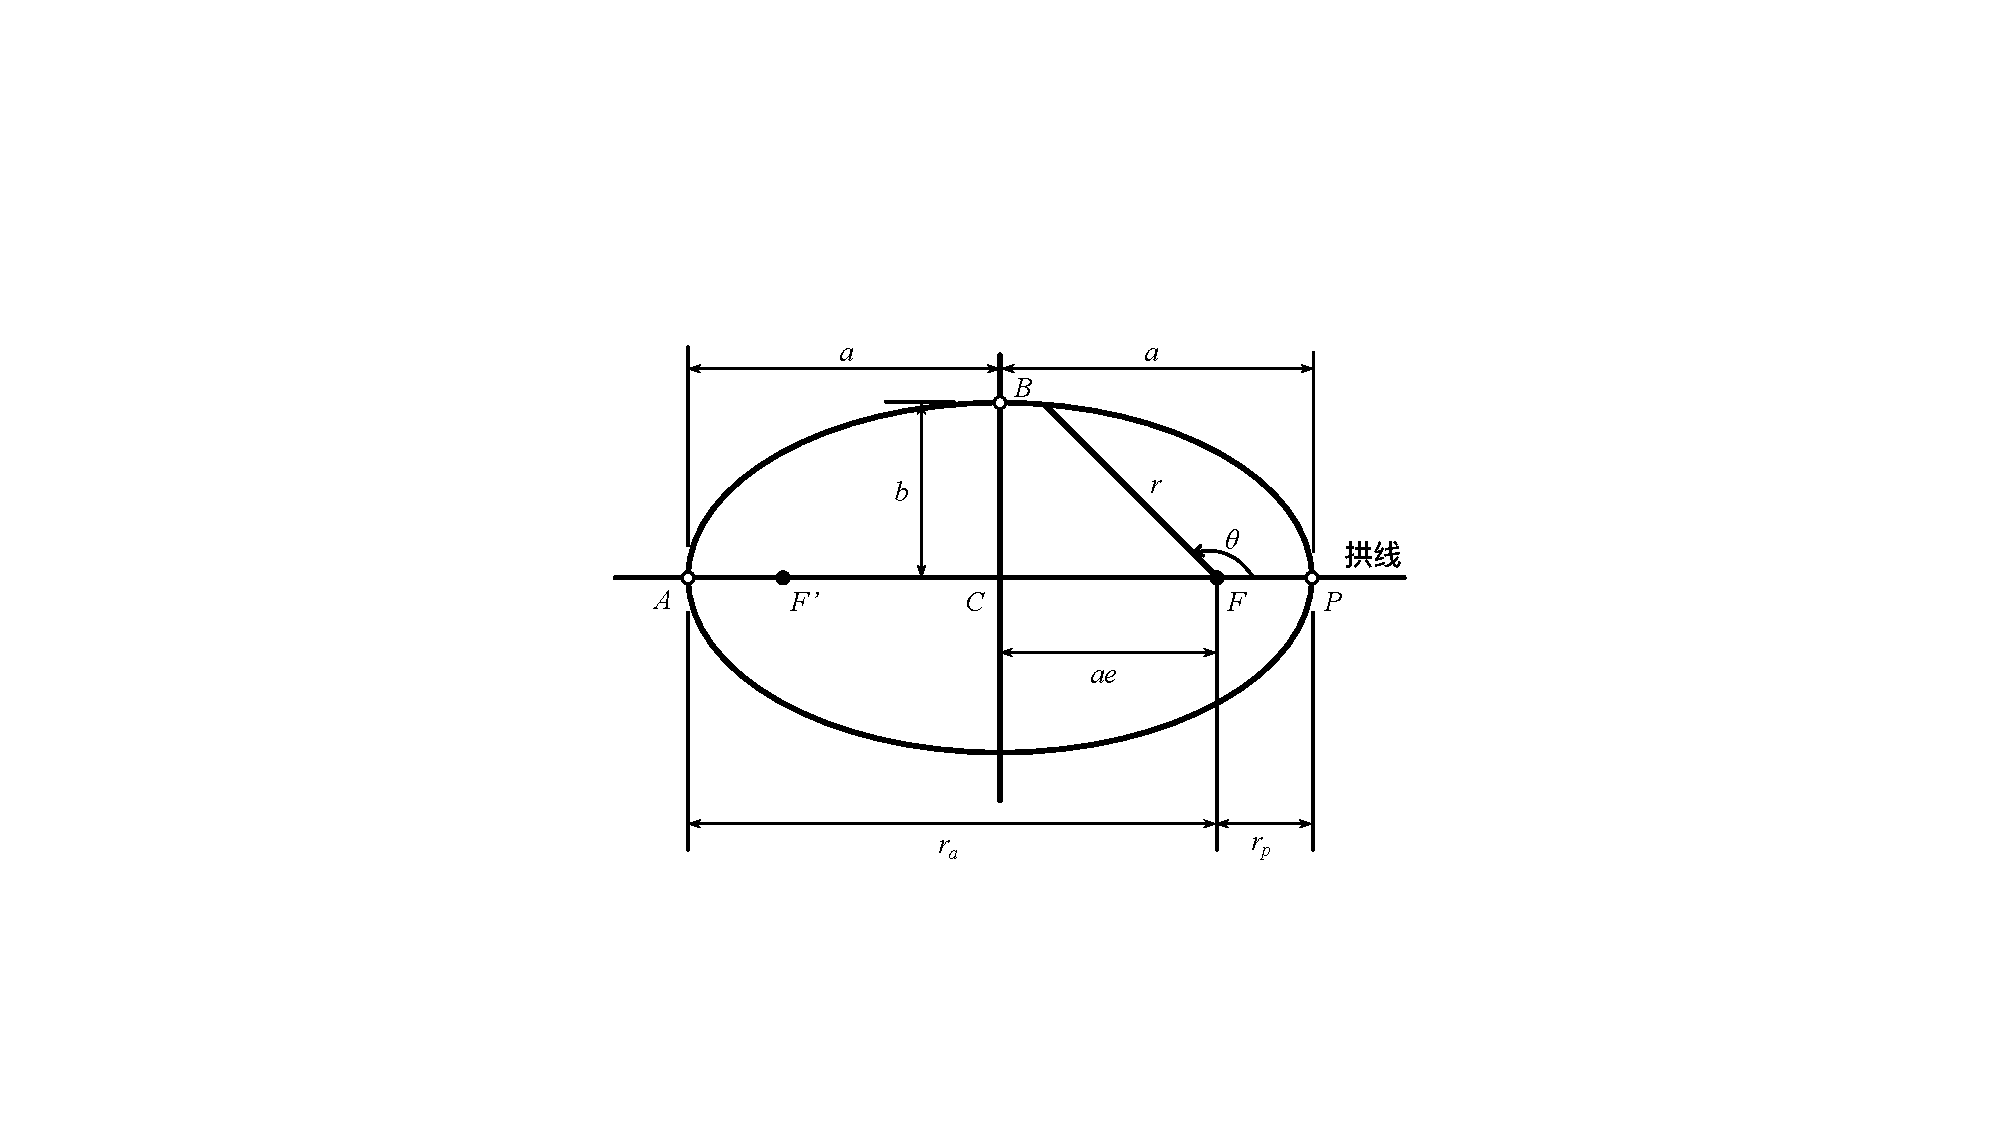
\includegraphics[width=0.8\linewidth]{pic/椭圆.pdf}
		\vspace*{-0.5em}
		\caption{椭圆轨道示意图}
		\label{椭圆}
	\end{minipage}
	\begin{minipage}{0.45\linewidth}
		\centering
		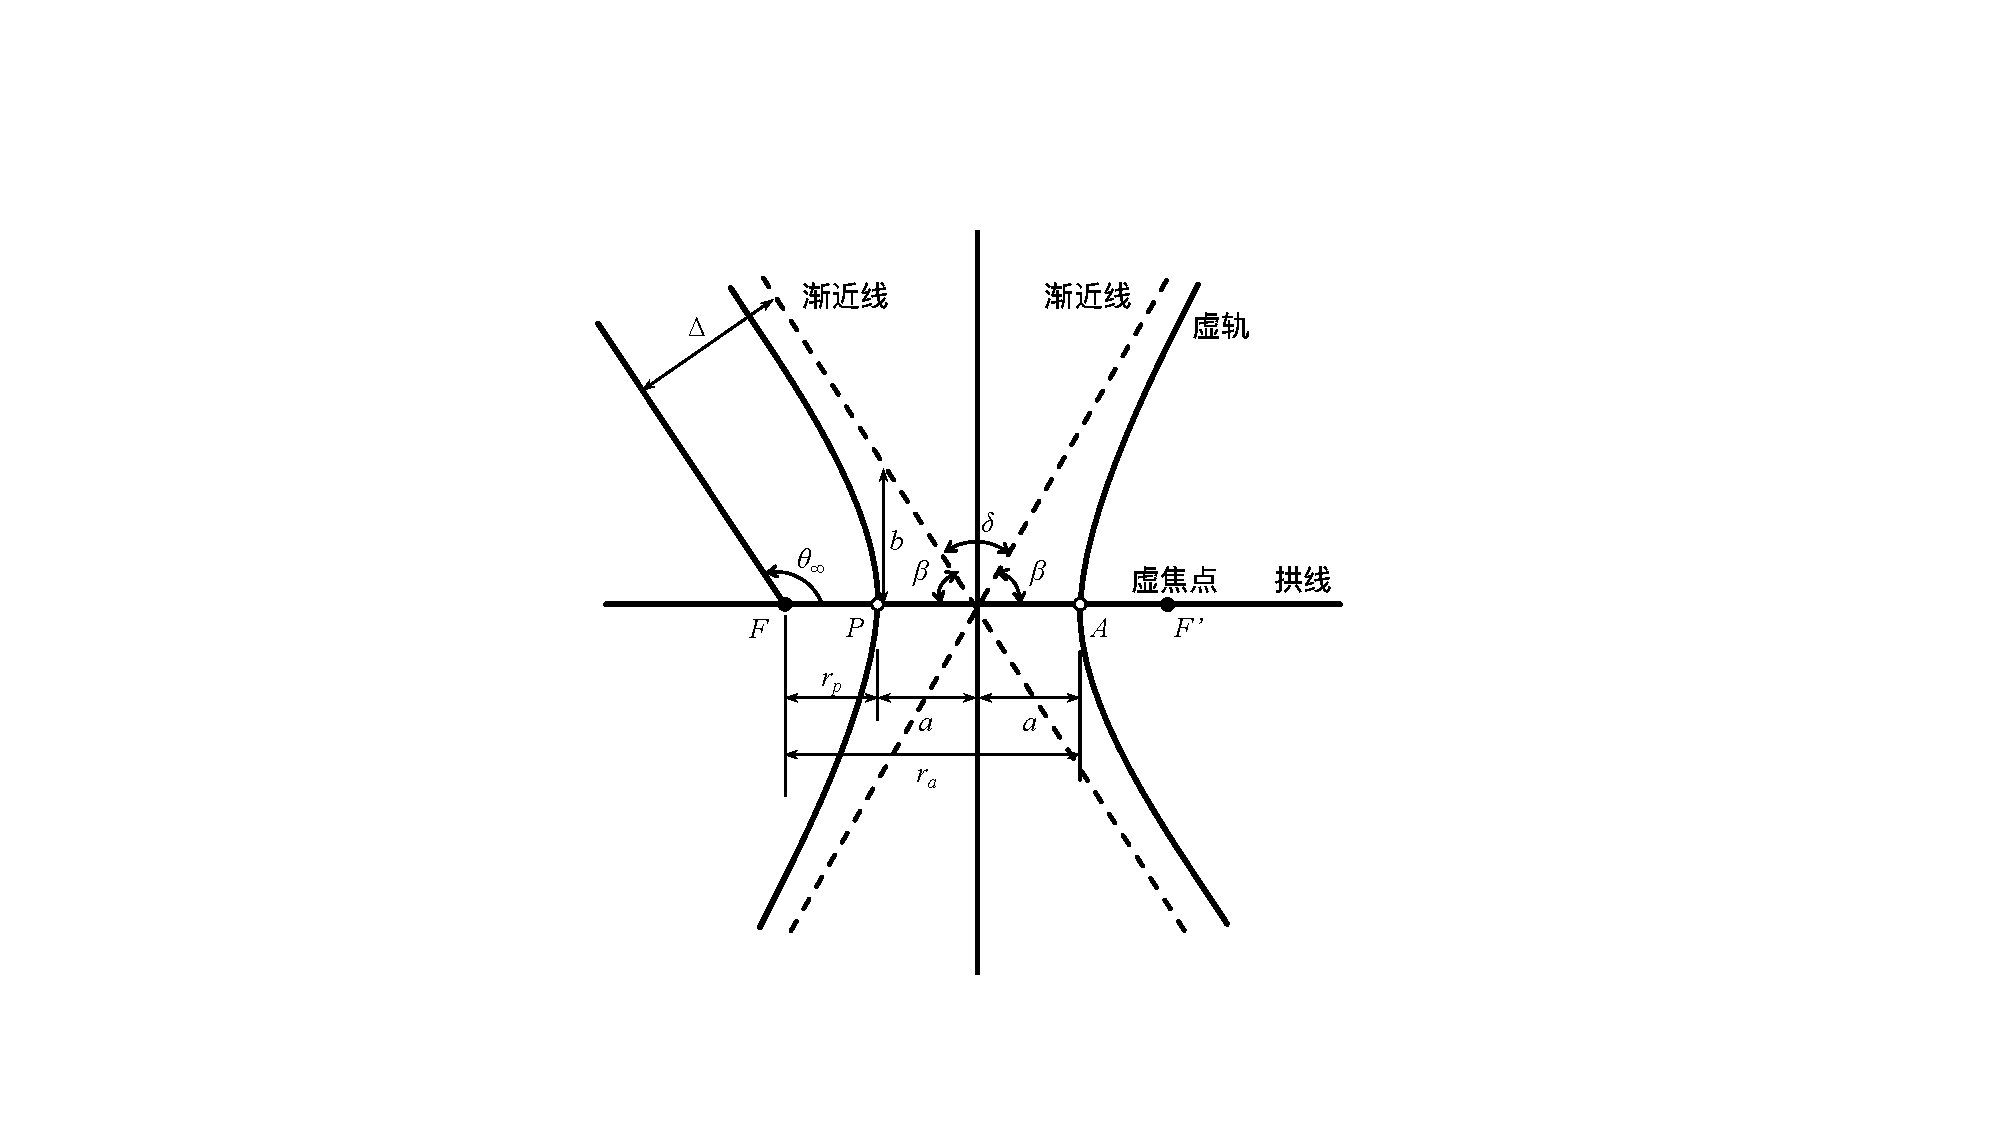
\includegraphics[width=\linewidth]{pic/双曲线.pdf}
		\vspace*{-2em}
		\caption{双曲线轨道示意图}
		\label{双曲线}
	\end{minipage}
\end{figure}
\vspace*{-1em}

\subsection{抛物线轨道($e = 1$)}
\begin{table}[!htb]
	\centering
	\setlength{\tabcolsep}{7mm}{
		\begin{tabular}{clcl}
			\hline
			&&&\\[-1.1em]
			离心率 & $\displaystyle e = 1$ &   飞行路径角  &  $\displaystyle \tan \gamma =  \dfrac{\sin \theta}{1 +  \cos \theta} \, \Rightarrow \, \gamma = \dfrac{\theta}{2} $ \\
			&&&\\[-1.1em]
			\hline
			&&&\\[-1.1em]
			轨道半径 & $\displaystyle r = \dfrac{h^2}{\mu} \dfrac{1}{1 + \cos \theta}$ & (逃逸)速度 & $v = \sqrt{\dfrac{2 \mu}{r}}$ \\
			&&&\\[-1.1em]
			\hline
			&&&\\[-0.8em]
			径向速度 & $\displaystyle v_r =  \dfrac{\mu}{h} \sin \theta$ & 切向速度 & $\displaystyle  v_{\bot} = \dfrac{\mu}{h}(1 + \cos \theta)$ \\
			&&&\\[-1em]
			\hline
			&&&\\[-1.1em]
			轨道周期 &无($\theta \to 180\degree, \, r \to \infty$)& 轨道能量 & $\varepsilon = -\dfrac{1}{2} \dfrac{\mu}{h^2}(1 - e^2) = 0$ \\[0.7em]
			\hline
		\end{tabular}
	}
	\caption{抛物线轨道的各个参数}
	\label{抛物线1}
\end{table}

\subsection{双曲线轨道($e > 1$)}

\begin{table}[!htb]
	\centering
	\setlength{\tabcolsep}{3.5mm}{
		\begin{tabular}{clcl}
			\hline
			&&&\\[-1.2em]
			短半轴 & $\displaystyle a = \dfrac{r_a + r_p}{2} = \dfrac{h^2}{\mu} \dfrac{1}{e^2 - 1}$ & 长半轴 & $\displaystyle b = a \sqrt{e^2 - 1}$ \\
			&&&\\[-1.2em]
			\hline
			&&&\\[-1.2em]
			远地点 & $\displaystyle r_a = \dfrac{h^2}{\mu} \dfrac{1}{1 - e} = -a (e + 1)$ & 近地点 & $\displaystyle r_p = \dfrac{h^2}{\mu} \dfrac{1}{1 + e} = a (1 - e)$ \\
			&&&\\[-1.2em]
			\hline
			&&&\\[-1.2em]
			转向角 & $\displaystyle \sin \dfrac{\delta}{2} = \sin(90\degree - \beta) = \cos \beta = \dfrac{1}{e}$ & 准径 & $\displaystyle \Delta = a \sqrt{e^2 - 1}$ \\
			&&&\\[-1.2em]
			\hline
			&&&\\[-1.2em]
			轨道半径 & $\displaystyle r = \dfrac{h^2}{\mu} \dfrac{1}{1 + e \cos \theta} = \dfrac{a(e^2 - 1)}{1 + e \cos \theta}$ & 速度 & $\displaystyle  v^2 = v_r^2 + v_{\bot}^2 = \dfrac{\mu^2}{h^2}(e^2 + 2e\cos \theta + 1)$ \\
			&&&\\[-1.2em]
			\hline
			&&&\\[-0.8em]
			径向速度 & $\displaystyle v_r =  \dfrac{\mu}{h}e \sin \theta$ & 切向速度 & $\displaystyle  v_{\bot} = \dfrac{\mu}{h}(1 + e \cos \theta)$ \\
			&&&\\[-1em]
			\hline
			&&&\\[-1.1em]
			 轨道周期 &无($\theta \to \theta_\infty, \, r \to \infty$)& 轨道能量 & $\varepsilon = -\dfrac{1}{2} \dfrac{\mu}{h^2}(1 - e^2) = - \dfrac{\mu}{2a}$  \\[0.8em]
			\hline
		\end{tabular}
	}
	\caption{双曲线轨道的各个参数}
	\label{双曲线1}
	\vspace*{-1.5em}
\end{table}

\clearpage

\begin{figure}[!htb]
	\centering
	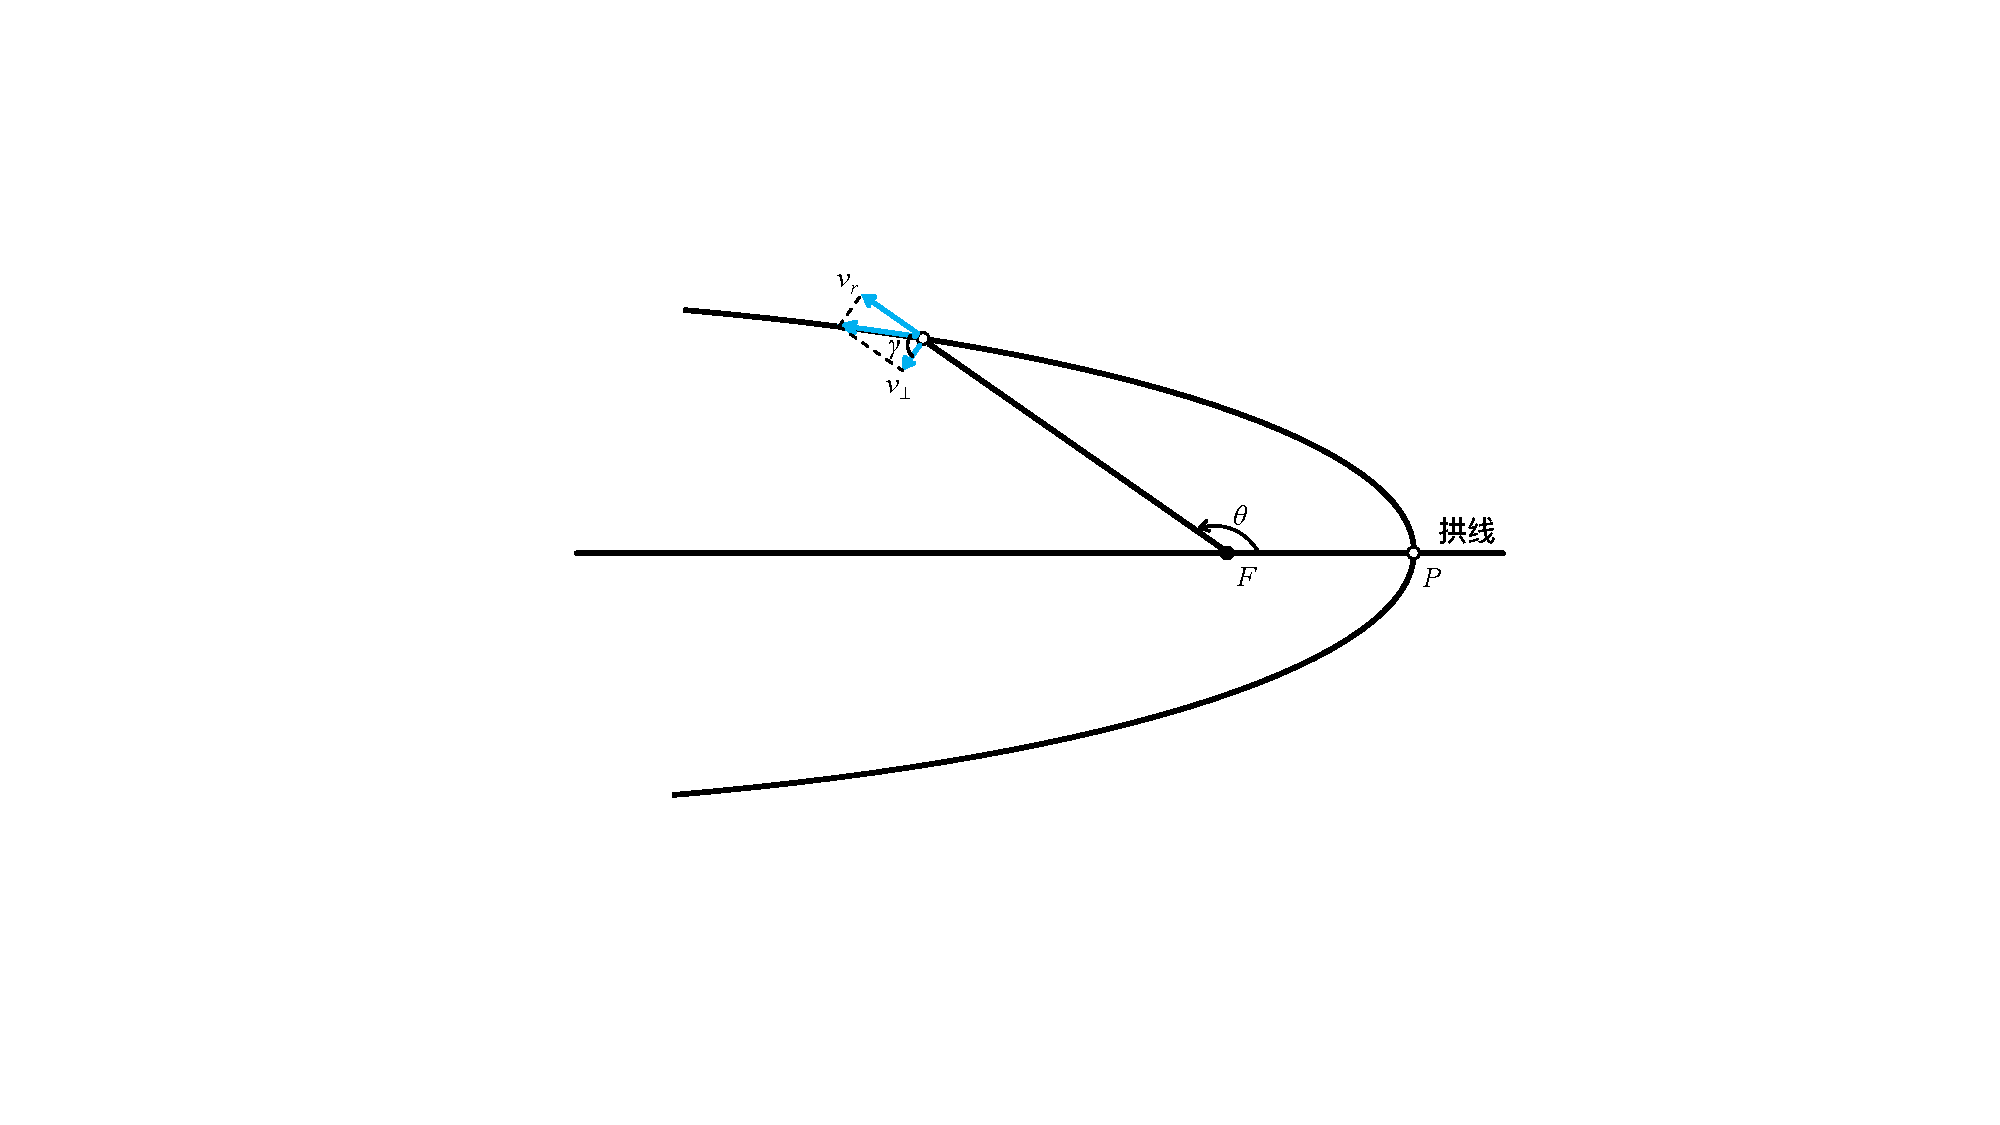
\includegraphics[width=0.55\linewidth]{pic/抛物线.pdf}
	\caption{抛物线示意图}
\end{figure}

双曲线的飞行路径角按照统一的公式计算:
\begin{equation}
	\tan \gamma = \dfrac{e \sin \theta}{1 + e \cos \theta}
\end{equation}
极限角$\theta_{\infty}$为
\begin{equation}
	\sin \theta_{\infty} = \dfrac{\sqrt{e^2 - 1}}{e}
\end{equation}

\subsection{剩余速度}
\hspace*{2em} 在三种轨道类型中,只有双曲线轨道的轨道能量是正值,则定义剩余速度为
\begin{equation}
	v_{\infty} = \sqrt{\dfrac{\mu}{a}} = \dfrac{\mu}{h}\sqrt{e^2 - 1}
\end{equation}
代表航天器超出中心引力逃逸所需要的能量,则双曲线轨道的速度可以写为
\begin{equation}
v^2 = v_{\text{\scriptsize \mbox{逃逸}}}^2 + v_{\infty}^2	
\end{equation}
记特征能量为
\begin{equation}
	C_3 = v_{\infty}^2
\end{equation}
设计火箭的特征能量要比其任务所需的特征能量大,以防突发情况。

\hspace*{2em} 抛物线是在无穷远闭合的轨道,是能量为负值的椭圆轨道和非闭合且轨道能量为正值的双曲线轨道之间的分界线。


\end{document}
